\section{Grupo Cociente}%
\label{sec:Grupo Cociente}

\begin{defi}[Producto de Subgrupos]
	Sea $(G, \circ, e)$ un grupo, sean $S, T \le G$, definimos el producto de $S$ y $T$ como:
	\begin{equation*}
		ST = \{ st : s \in S, t \in T \}
	\end{equation*}
\end{defi}

\ObservacionBox{}{
	Sea $(G, \circ, e)$ un grupo, $S, T \subseteq G$, $ST$, no es necesariamente un subgrupo.
}

\begin{prop}
	Sea $(G, \circ, e)$ un grupo, sean $H, K \le G$ entonces $HK$ es un subgrupo si y sólo si $HK = KH$.
\end{prop}

\begin{proof}
	\textbf{$\Rightarrow$)} Suponga que $HK \le G$, sean $hk \in HK$, entonces $h \in H$ y $k \in K$, entonces:
	$k^{-1}h^{-1} = (hk)^{-1} \in HK$, por otro lado, como $k^{-1}h^{-1} \in KH$, así: $HK = (k^{-1}h^{-1})^{-1} \in KH$, luego $HK \subseteq KH$, análogamente $KH \subseteq HK$, por lo tanto $HK = KH$.

	\textbf{$\Leftarrow$)} Supongamos que $HK = KH$, notemos que $HK \neq \emptyset$, ya que $e \circ e \in HK$.
	Sean $x, y \in HK$, entonces existe $h_1, h_2 \in H, k_1, k_2 \in K$, tal que $x = h_1 k_1$, $y = h_2 k_2$, es claro que $y^{-1} \in HK$, pues $y^{-1} = k_2^{-1}h_2^{-1} \in KH = HK$, así que probemos que $x y^{-1} \in HK$. En efecto,
	$x y^{-1} = h_1 k_1 (h_2 k_2)^{-1} = h_1 k_1 k_2^{-1}h_2^{-1}$.
	Note que $k_1 k_2^{-1}h_2^{-1} \in KH = HK$, entonces digamos $h_3 k_3 = k_1 k_2^{-1}h_2^{-1}$ con $h_3 \in H, k_3 \in K$.
	Luego:
	$h_1(k_1 k_2^{-1}h_2^{-1}) = h_1(h_3 k_3) \in HK$, por lo tanto $xy^{-1} \in HK$, y por una proposición anterior $HK$ es un subgrupo de $G$.
\end{proof}

\begin{defi}
	Sea $(G, \circ, e)$ un grupo, sean $H, K \le G$, $HK$ se llama el producto de $H$ con $K$.
\end{defi}

\CorolarioBox{}{
	Si $(G, \circ, e)$ es un grupo abeliano el producto finito de subgrupos es un subgrupo.
}

\begin{enefecto}
	es inmediato usando inducción y el hecho que el producto de subgrupos es asociativo.
\end{enefecto}

\ObservacionBox{}{
	Sea $(G, \circ, e)$ un grupo, sea $H \le G$, entonces $Hg = H$ si y sólo si $g \in H$.
}

\begin{proof}
	\textbf{$\Rightarrow$)} Supongamos que $Hg = H$, entonces $\forall hg \in Hg, hg \in H$, en particular tome $h=e$, así $eg = g \in H$.

	\textbf{$\Leftarrow$)} Suponga que $g \in H$, entonces $Hg = \{ hg : h \in H \} \subseteq H$, ahora dado $h \in H$, note que $hg^{-1} \in H$, luego $h = (hg^{-1})g \in Hg$, por lo cual $H \subseteq Hg$.
	$\therefore Hg = H$.
\end{proof}

\begin{prop}
	Sea $(G, \circ, e)$ un grupo, $H \le G$, entonces $Hg = Hg_1$ si y sólo si $gg_1^{-1} \in H$.
\end{prop}

\begin{enefecto}
	$gg_1^{-1} \in H \iff H = Hgg_1^{-1} \iff Hg_1 = (Hgg_1^{-1})g_1 = Hg$.
\end{enefecto}

\begin{defi}
	Sea $(G, \circ, e)$ un grupo, sea $H \le G$, sea $g \in G$, a $Hg$ se le llama clase derecha, análogamente $gH$ se le llama clase izquierda.
\end{defi}

\begin{defi}
	Sea $(G, \circ, e)$ un grupo, sea $H \le G$, sea $\mathcal{L} = \{ gH : g \in G \}$ se le llama conjunto de clases izquierdas y $\mathcal{R} = \{ Hg : g \in G \}$ se le llama conjunto de clases derechas.
\end{defi}

\begin{prop}
	Sea $(G, \circ, e)$ un grupo, sea $H \le G$, entonces $\mathcal{L}$ y $\mathcal{R}$ forman una partición de $G$.
\end{prop}

\begin{proof}
	Basta probar que $\mathcal{R}$ induce una relación de equivalencia, i.e. la relación $\sim$ definida por $a \sim b \iff a, b \in Hg$ es de equivalencia.
	\begin{enumerate}[label=\roman*), font=\normalfont]
		\item \textsc{Reflexividad:} $a \sim a \iff a, a \in Hg$. (Esto se cumple pues $a \in Ha$).
		\item \textsc{Simétrica:} $a \sim b \implies a, b \in Hg \implies b, a \in Hg \implies b \sim a$.
		\item \textsc{Transitividad:} Si $a \sim b \land b \sim c \implies a, b \in Hg_1 \land b, c \in Hg_2$.
		      Sea $a = h_1 g_1$, $b = h_2 g_1$, $b = h_3 g_2$, $c = h_4 g_2$, así note que $g_1 = (h_2^{-1} h_3) g_2$.
		      Luego podemos expresar $a = h_1 (h_2^{-1} h_3) g_2$, como $(h_1 h_2^{-1} h_3) \in H$, $a \in Hg_2$, así $a, c \in Hg_2 \implies a \sim c$.
	\end{enumerate}

	$\therefore$ Las clases derechas forman una partición de $G$.

	Análogamente las clases izquierdas forman una partición de $G$.
\end{proof}

\ObservacionBox{}{
	Si $(G, \circ, e)$ es abeliano cada clase izquierda es la misma clase derecha.
}

\begin{enefecto}
	Sea $H \le G$, sea $\mathcal{L} = \{ gH : g \in G \}$, sea $\mathcal{R} = \{ Hg : g \in G \}$, sea $Hg \in \mathcal{R}$, sea $hg \in Hg$, $hg = gh \in gH \in \mathcal{L}$, así $\mathcal{R} \subseteq \mathcal{L}$, análogamente $\mathcal{L} \subseteq \mathcal{R}$, por lo cual $\mathcal{L} = \mathcal{R}$.
\end{enefecto}

\ObservacionBox{}{
	El recíproco es no necesariamente cierto.
}

\begin{eje}
	En $S_3$, sea $H = \left\{ \sigma = \begin{pmatrix} 1 & 2 & 3 \\ 2 & 1 & 3 \end{pmatrix}, e \right\} = \langle \sigma \rangle \le G$.

	Veamos cuáles son las clases derechas de $H$:
	\begin{equation*}
		\mathcal{R} = \{ H, H\theta = \{ \theta, \sigma \circ \theta \}, H\theta^2 = \{ \theta^2, \sigma \circ \theta^2 = \theta \circ \sigma \} \}
	\end{equation*}

	Ahora las clases izquierdas:
	\begin{equation*}
		\mathcal{L} = \{ H, \theta H = \{ \theta, \theta \circ \sigma \}, \theta^2 H = \{ \theta^2, \theta^2 \circ \sigma \} \}
	\end{equation*}
\end{eje}

\begin{prop}
	Sea $(G, \circ, e)$ un grupo, entonces la cardinalidad de cada clase izquierda o derecha es la misma e igual a $|H|$.
\end{prop}

\begin{proof}
	Sea $Hg \in \mathcal{R}$, definamos $\varphi: H \to Hg$, $h \mapsto hg$, probemos que es una función biyectiva.

	En efecto, sean $h_1, h_2 \in H$, tal que $\varphi(h_1) = \varphi(h_2)$, entonces $h_1 g = h_2 g \iff h_1 = h_2$, por lo tanto es inyectiva.

	Sea $hg \in Hg \implies \exists h \in H$ tal que $\varphi(h) = hg$, por lo tanto es suprayectiva.

	$\therefore \varphi$ es biyectiva, así $|H| = |Hg|$. Análogamente se prueba que $|H| = |gH|$.
\end{proof}

\TeoremaBox{Índice de Lagrange}{
	Sea $(G, \circ, e)$ un grupo sea $H \le G$, entonces $|H| \mid |G|$ y además:
	\begin{equation*}
		|G| = |H| \cdot [G:H]
	\end{equation*}
}

Donde $[G:H] := |\mathcal{L}| = |\mathcal{R}|$ se llama índice de Lagrange de $H$ en $G$.

\begin{proof}
	Primero veamos que $|\mathcal{L}| = |\mathcal{R}|$. Sea $\varphi: \mathcal{R} \to \mathcal{L}$, $Ha \mapsto a^{-1}H$, probemos que es un isomorfismo (biyeción entre conjuntos).

	Sean $g_1 H, g_2 H \in \mathcal{R}$, tal que $\varphi(Hg_1) = \varphi(Hg_2)$, entonces:
	\begin{equation*}
		g_1^{-1} H = g_2^{-1} H \iff g_1 (g_2^{-1})^{-1} \in H \iff g_1 g_2^{-1} \in H \iff Hg_1 = Hg_2
	\end{equation*}
	Por lo tanto es inyectiva. (Nota: en la imagen la cadena de equivalencias usa propiedades de clases laterales).

	Ahora sea $g^{-1}H \in \mathcal{L}$, como existe $g=(g^{-1})^{-1} \in G$, se sigue que $\exists Hg \in \mathcal{R}$, tal que $\varphi(Hg) = g^{-1}H$, por lo cual es biyectiva.

	$\therefore \varphi$ es biyectiva y así es un isomorfismo (de conjuntos).
	$\therefore |\mathcal{R}| = |\mathcal{L}|$.

	Ahora como las clases son una partición de $G$, entonces:
	\begin{align*}
		|G| & = \left| \bigcup_{a \in G} Ha \right|      \\
		    & = \sum_{a \in G} |Ha| = \sum_{a \in G} |H| \\
		    & = |\mathcal{R}| |H| = |H| [G:H]
	\end{align*}

	Así: $|H| \mid |G|$ y $[G:H] \mid |G|$.
\end{proof}

En particular si $G$ es finito, se cumple que:
\begin{equation*}
	\frac{|G|}{|H|} = [G:H]
\end{equation*}

\begin{defi}
	Sea $(G, \circ, e)$ un grupo, sea $g \in G$, se denota por $o(g)$ como el menor entero no negativo tal que $g^{o(g)} = e$, si existe ese entero, en caso contrario, diremos $o(g) = +\infty$.
\end{defi}

\begin{eje}
	En $(\mathbb{Z}, +, 0)$, $\forall a \in \mathbb{Z}, \quad o(a) = 0$ (o infinito según la convención).
\end{eje}

\begin{eje}
	En $(S_3, \circ, e) \quad o(\sigma) = 2, \quad o(\theta) = 3$.
\end{eje}

\begin{eje}
	En $(\mathbb{Z}/8\mathbb{Z}, +, 0), \quad o(2)=4, \quad o(3)=8, \quad o(4)=2$.
\end{eje}

\ObservacionBox{}{
	Sea $(G, \circ, e)$ un grupo finito $\forall g \in G, \exists m \in \mathbb{Z}^+$, tal que $o(g) \le m$.
}

\begin{proof}
	Sea $|G|=n$, tome el conjunto $\{g^{i_1}, \dots, g^{i_{n+1}}\}$, con $i_1, \dots, i_{n+1} \in \mathbb{Z}^+$ con $i_1 < i_2 < \dots < i_{n+1}$. Entonces al menos 2 son iguales, i.e. $g^{i_j} = g^{i_k}$, para $1 \le j < k \le n+1$.
	Luego:
	\begin{equation*}
		g^{i_k - i_j} = g^{i_k} \cdot g^{-i_j} = g^{i_j} g^{-i_j} = e, \quad \text{tomemos } m = i_k - i_j > 0.
	\end{equation*}
	$\therefore \exists m \in \mathbb{Z}^+$ tal que $g^m = e$, luego como $o(g)$ es el mínimo entero positivo tal que $g^{o(g)} = e$, entonces $o(g) \le m$.
\end{proof}

\ObservacionBox{}{
	Sea $(G, \circ, e)$ un grupo finito, sea $g \in G$, $o(g) = |\langle g \rangle|$, más aún $o(g) \mid |G|$.
}

\begin{proof}
	Sea $H = \{ e, g, g^2, \dots, g^{o(g)-1} \}$, claramente $H \subseteq \langle g \rangle$, además notemos que es un subgrupo.

	En efecto: sean $g^i, g^j \in H, \quad 0 \le i < j \le o(g)-1$, entonces $g^i g^j = g^{i+j}$, se tiene que $0 \le i+j \le o(g)-1 \lor o(g) \le i+j$. Si se cumple la primera condición es evidente que $g^{i+j} \in H$.
	Por lo cual tomemos el caso $o(g) \le i+j$, por el algoritmo de Euclides $\exists k, r \in \mathbb{Z}^+$ tal que:
	$i+j = k \cdot o(g) + r$, con $0 \le r < o(g)$, así:
	\begin{equation*}
		g^{i+j} = g^{k \cdot o(g) + r} = (g^{o(g)})^k g^r = (e)^k g^r = g^r \in H,
	\end{equation*}
	por lo tanto es cerrada, además se hereda de $G$ las propiedades del grupo.

	Ahora sea $a \in \langle g \rangle$, podemos expresar $a = g^i, i \in \mathbb{Z}$, así por Euclides $\exists k, r \in \mathbb{Z}$, con $0 \le r < o(g)$ tal que $g^i = o(g)k + r$, de este modo podemos expresar $a = g^i = g^r \in H$.

	$\therefore \langle g \rangle \subseteq H$, así $|\langle g \rangle| = |H| = o(g)$, más aún como $H$ es subgrupo de $G$, $|H| \mid |G|$, así $o(g) \mid |G|$.
\end{proof}

\CorolarioBox{}{
	Sea $(G, \circ, e)$ un grupo finito entonces $g^{|G|} = e \quad \forall g \in G$.
}

\begin{proof}
	Dado que $o(g) = |\langle g \rangle| \mid |G|$, entonces $\exists s$ tal que $o(g)s = |G|$ y
	\begin{equation*}
		g^{|G|} = g^{o(g)s} = (g^{o(g)})^s = (e)^s = e
	\end{equation*}
\end{proof}

\CorolarioBox{Teorema de Euler}{
	Sea $a \in (\mathbb{Z}/n\mathbb{Z})^*$ entonces $a^{\varphi(n)} = 1 \pmod n$.
}

\begin{proof}
	$|(\mathbb{Z}/n\mathbb{Z})^*| = \varphi(n)$ y por el corolario anterior
	\begin{equation*}
		a^{\varphi(n)} = 1 \pmod n
	\end{equation*}
\end{proof}

\CorolarioBox{Teorema Pequeño de Fermat}{
	Si $a \in (\mathbb{Z}/p\mathbb{Z})^*$ con $p$ primo, entonces: $a^p \equiv a \pmod p$ y $a^{p-1} = 1$.
}

\begin{enefecto}
	Por el corolario anterior dado $a \in (\mathbb{Z}/p\mathbb{Z})^*$, $a^{\varphi(p)} = 1 \pmod p$, como $\varphi(p) = p-1$, se sigue $a^{p-1} = 1 \pmod p$, luego $a^p = a$.
\end{enefecto}

\begin{defi}
	Sea $(G, \circ, e)$ un grupo sea $N \le G$, diremos que $N$ es un subgrupo normal en $G$ denotado por $N \trianglelefteq G$, si $gNg^{-1} = N, \forall g \in G$.
\end{defi}

\ObservacionBox{}{
	Si $(G, \circ, e)$ es un grupo, sea $N \subseteq G$, arbitrario entonces $gNg^{-1} \subseteq G$. En este caso diremos que $gNg^{-1}$ es subgrupo conjugado de $N$.
}

\begin{enefecto}
	Es claro que $gNg^{-1} \neq \emptyset$ pues $N \neq \emptyset$. Además para $h_1, h_2 \in gNg^{-1}$, $\exists n_1, n_2 \in N$ tal que $h_1 = g n_1 g^{-1}$, $h_2 = g n_2 g^{-1}$, luego:
	\begin{equation*}
		h_1 h_2^{-1} = g n_1 g^{-1} (g n_2 g^{-1})^{-1} = g n_1 g^{-1} (g^{-1})^{-1} n_2^{-1} g^{-1} = g n_1 n_2^{-1} g^{-1} \in gNg^{-1}
	\end{equation*}
	$\therefore$ es un subgrupo de $G$.
\end{enefecto}

\TeoremaBox{}{
	Sea $(G, \circ, e)$ un grupo, $N \le G$, entonces las siguientes condiciones son equivalentes:
	\begin{enumerate}[label=\roman*), font=\normalfont]
		\item $N \trianglelefteq G$.
		\item $gNg^{-1} \subseteq N \quad \forall g \in G$.
		\item $gNg^{-1} = N \quad \forall g \in G$. (Nota: en la imagen dice $gN \subseteq Ng$, pero el punto iii suele referirse a la igualdad de conjugación o conmutación de clases. Transcribo lo que dice la imagen literalmente en la demostración: $gNg^{-1} \subseteq N \implies gN \subseteq Ng$).
		\item $gN = Ng \quad \forall g \in G$.
		\item El único subgrupo conjugado de $N$ es $N$.
	\end{enumerate}
}

\newpage
\begin{proof}

	\begin{itemize}
		\item \textsc{i} $\Rightarrow$ \textsc{ii}) De la definición $gNg^{-1} = N \quad \forall g \in G$, en particular $gNg^{-1} \subseteq N \quad \forall g \in G$.
		\item \textsc{ii} $\Rightarrow$ \textsc{iii}) $gNg^{-1} \subseteq N \implies (gNg^{-1})g \subseteq Ng$ y $g(gNg^{-1}) = gN$, así $gN \subseteq Ng \quad \forall g \in G$.
		      (Nota: Aquí la transcripción se ajusta a la lógica del manuscrito que parece deducir la igualdad de clases o contención).
		\item \textsc{iii} $\Rightarrow$ \textsc{iv}) Resta ver que $Ng \subseteq gN$. Tenemos que $gN \subseteq Ng \quad \forall g \in G$, se sigue:
		      $g^{-1}N \subseteq Ng^{-1} \quad \forall g \in G \implies g(g^{-1}N) \subseteq gNg^{-1} \implies N \subseteq gNg^{-1} \quad \forall g \in G$, así:
		      $Ng \subseteq (gNg^{-1})g = gN \quad \forall g \in G$.
		\item \textsc{iv} $\Rightarrow$ \textsc{v}) Sea $H$ el conjugado de $N$ entonces $H = gNg^{-1}$ para algún $g \in G$, entonces:
		      \begin{equation*}
			      Hg = (gNg^{-1})g = gN = Ng
		      \end{equation*}
		      de donde
		      \begin{equation*}
			      H = (Hg)g^{-1} = (Ng)g^{-1} = N
		      \end{equation*}
		\item \textsc{v} $\Rightarrow$ \textsc{i}) Se sigue de la definición.
	\end{itemize}

\end{proof}

\ObservacionBox{}{
	Si $N \trianglelefteq G$ y $H \le G$ entonces $HN = NH$ y por tanto $NH \le G$.
}

\begin{enefecto}
	$HN = \bigcup_{h \in H} hN = \bigcup_{h \in H} Nh = NH$.
\end{enefecto}

\begin{eje}
	Dado el grupo $S_3$, calcule los subgrupos: $S_3 = \{e, \sigma, \theta, \theta^2, \sigma\theta, \theta\sigma\}$
\end{eje}
\textit{ Sol. }
\begin{align*}
	H_0 & = \langle e \rangle = \{e\}                                                  \\
	H_1 & = \langle \sigma \rangle = \{e, \sigma\}                                     \\
	H_2 & = \langle \theta \rangle = \{e, \theta, \theta^2\} = \{e, \theta^2, \theta\} \\
	H_3 & = \langle \sigma \circ \theta \rangle = \{e, \sigma \circ \theta\}           \\
	H_4 & = \langle \theta \circ \sigma \rangle = \{e, \theta \circ \sigma\}           \\
	H_5 & = \langle \{\sigma, \theta\} \rangle = S_3
\end{align*}
Además podemos notar:
\begin{itemize}
	\item $H_0 \trianglelefteq G$, de manera trivial.
	\item $H_1 \not\trianglelefteq G$, ya que $H_1 \theta \neq \theta H_1$.
	\item $H_2 \trianglelefteq G$, $H_2 \sigma = \{\sigma, \theta \circ \sigma, \theta^2 \circ \sigma\} = \{\sigma, \theta \circ \sigma, \sigma \circ \theta\} = \sigma H_2$.
	\item $H_3 \not\trianglelefteq G$, $H_3 \theta \neq \theta H_3$.
	\item $H_4 \not\trianglelefteq G$, $H_4 \theta \neq \theta H_4$.
	\item $H_5 \trianglelefteq G$, ya que $H_5 = S_3$.
\end{itemize}

Por otro lado note:
\begin{align*}
	\theta H_1 \theta^{-1} & = \theta H_1 \theta^2 = \{e, \theta \circ \sigma \circ \theta^2\} = \{e, \theta \circ \theta \circ \sigma\} = \{e, \theta^2 \circ \sigma\} = \{e, \sigma \circ \theta\} = H_3. \\
	\theta H_3 \theta^{-1} & = \theta H_3 \theta^2 = \{e, \theta \circ (\sigma \circ \theta) \circ \theta^2\} = \{e, \theta \circ \sigma\} = H_4
\end{align*}

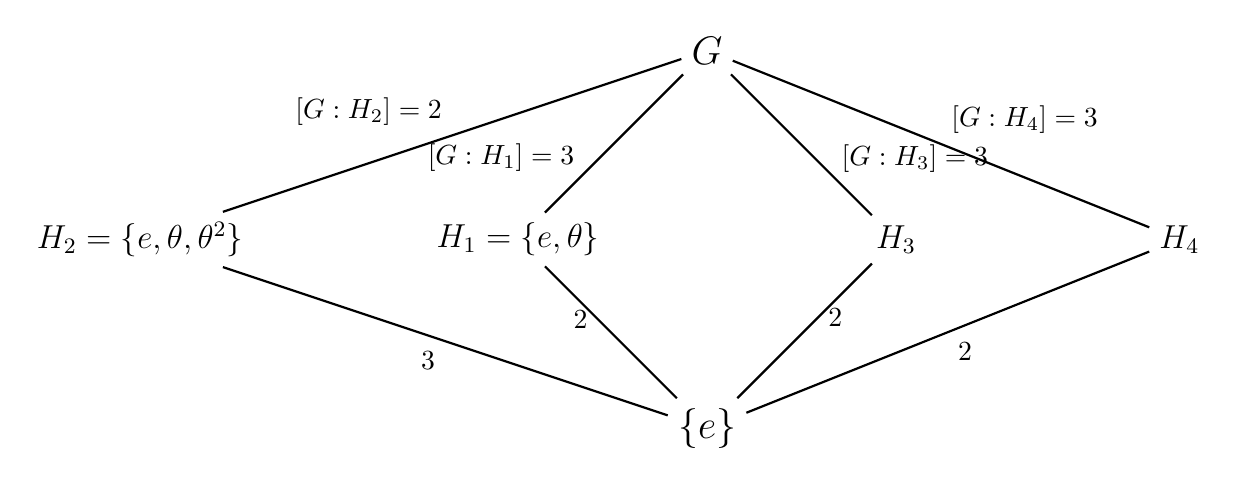
\begin{tikzpicture}[thick, scale=1.2]

	% 1. Definición de Nodos (Posiciones x, y)
	% Nodo superior
	\node (G) at (0, 4) {\Large $G$};

	% Nodos intermedios (ajustando coordenadas X para que quepan las fórmulas)
	\node (H2) at (-6, 2) {\large $H_2=\{e, \theta, \theta^2\}$};
	\node (H1) at (-2, 2) {\large $H_1=\{e, \theta\}$};
	\node (H3) at (2, 2) {\large $H_3$};
	\node (H4) at (5, 2) {\large $H_4$};

	% Nodo inferior
	\node (e) at (0, 0) {\Large $\{e\}$};

	% 2. Conexiones Superiores (De G a los subgrupos)
	% Usamos 'node' dentro de 'draw' para poner las etiquetas de índices
	\draw (G) -- node[above left] {$[G:H_2]=2$} (H2);
	\draw (G) -- node[left, pos=0.6, xshift=-0.2cm] {$[G:H_1]=3$} (H1);
	\draw (G) -- node[right, pos=0.6, xshift=0.2cm] {$[G:H_3]=3$} (H3);
	\draw (G) -- node[above right] {$[G:H_4]=3$} (H4);

	% 3. Conexiones Inferiores (De subgrupos a {e})
	\draw (H2) -- node[below left] {3} (e);
	\draw (H1) -- node[left, pos=0.4] {2} (e);
	\draw (H3) -- node[right, pos=0.4] {2} (e);
	\draw (H4) -- node[below right] {2} (e);

\end{tikzpicture}
